% Локализация маловероятных регионов и т.п.
\subsection{Векторизация с помощью удаления маловероятных регионов из плоского цикла}

\subsubsection{Вынос маловероятного региона из цикла}

\subsubsection{Эксперимент по применению выноса маловероятного региона для повышения эффективности векторизации}

\cite{Rybakov2017Flight,Rybakov2022VecGeom}

\subsubsection{Выделение вероятного пути исполнения с помощью оптимизации <<черная дыра>>}

В этом разделе описан метод выноса маловероятных регионов из плоского цикла в общем случае с помощью подхода, который в некоторых источниках применительно к своим предметным областям встречается под названием blackhole (<<черная дыра>>) \cite{Ilbeyi2019}.

\begin{figure}[ht]
	\centering
	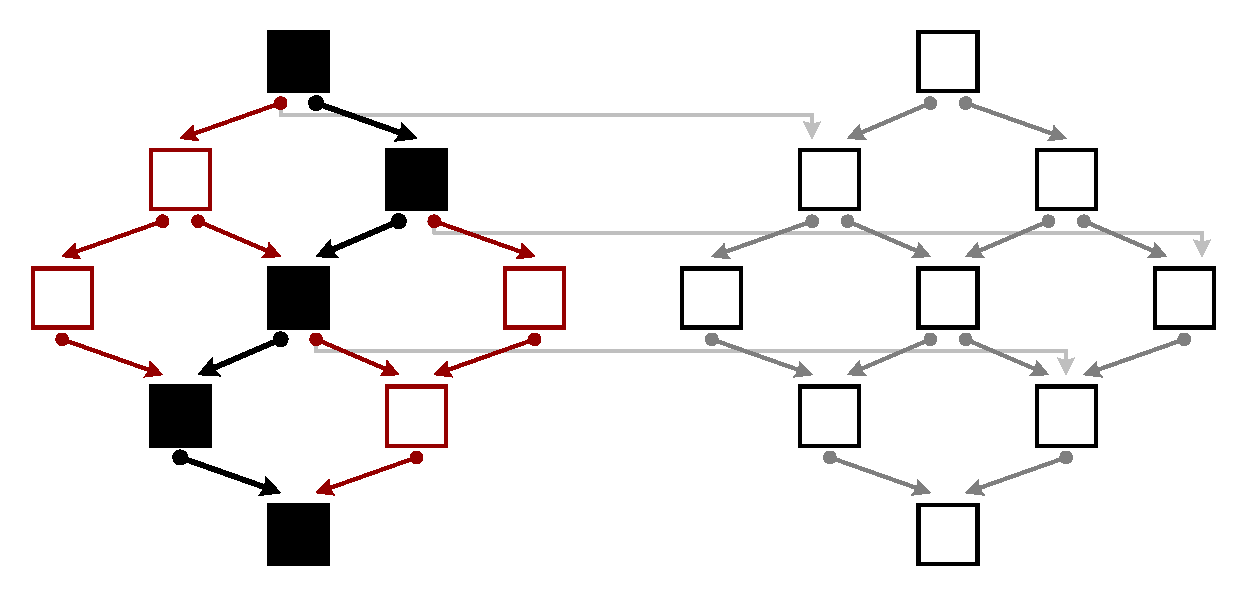
\includegraphics[width=1.0\textwidth]{./pics/text_4_vec_loc_branch/blackhole.pdf}
	\caption{Иллюстрация схемы работы оптимизации <<черная дыра>>.}
	\label{fig:text_4_vec_loc_branch_blackhole}
\end{figure}

Пусть дам некоторый CFG тела плоского цикла (рис.~\ref{fig:text_4_vec_loc_branch_blackhole} слева), в котором присутствует явно выделенный пусть исполнения (на рисунке выделен черным цветом), вероятность прохождения которого близка к единице \cite{Shabanov2021VecCFG}.
Другие крайне маловероятные линейные участки (выделенные на рисунке красным цветом) представляют собой программный контекст, который практически никогда не исполняется, и векторизацию которого проводить нецелесообразно, либо невозможно.
Оптимизация blackhole заключается в создании точной копии CFG, на которую перенаправляются все маловероятные переходы из основного тела.
После выполнения перенаправления маловероятных переходов все ребра и линейные участки, отмеченные на рис.~\ref{fig:text_4_vec_loc_branch_blackhole} красным цветом, могут быть удалены.
Таким образом, после выполнения оптимизации в качестве объекта векторизации остается ограниченный и пригодный к векторизации программный контекст.
В случае же если один из маловероятных переходов все же осуществится, то выполнится переход на точную копию изначального CFG, который хоть и не оптимально, но корректно отработает данную редкую ситуацию.
Эта оптимизация получила свое название blackhole потому что после выполнения редкого перехода на копию CFG программа не может вернуться обратно в векторизованную версию, в этом случае данный экземпляр плоского цикла закончит свое исполнение в <<черной дыре>>.
Оптимизация может применяться в различных вариациях.
Например, можно создавать копию не целого CFG, а только конкретных маловероятных регионов, в этом случае мы будем иметь оптимизацию локализации редких путей исполнения.
Наоборот, более консервативным вариантом оптимизации является перенаправление маловероятных переходов сразу на голову невекторизованной копии тела цикла, что соответствует просто проведению повторного расчета при возникновении исключительной ситуации.
